\documentclass[11pt]{article}

\usepackage[margin=1in]{geometry}
\usepackage{amsmath}
\usepackage{booktabs}
\usepackage{graphicx}
\usepackage{caption}
\usepackage{placeins}

\makeatletter
\setlength{\@fptop}{8pt}
\setlength{\@fpbot}{0pt plus 1fil}
\makeatother

\captionsetup{font=small,skip=8pt}
\setlength{\parskip}{0.45em}
\setlength{\parindent}{0pt}

\title{Stage 1: OU Estimates on a Static-OLS Hedge\\[0.3em]
\large 511090 against the TL future}
\date{29 September 2026}

\begin{document}
\maketitle

This note is stage 1 of the 511090--TL pair. The book trades a hedged residual and models that residual as an Ornstein--Uhlenbeck process. On the static residual, two estimates of the OU parameters are compared out of sample: a trailing OLS window, refreshed every 180 minutes, and a Kalman filter whose process noise and entry and exit bands were chosen on the training window.

\section{OU pair trading}
\label{sec:ou}

ETF 511090 and the TL future move together, and the book trades the residual left once one has been hedged with the other. The premise is that this residual returns to an equilibrium level. Above that level the book sells the residual; below it, the book buys the residual; once the residual is back inside a band, the book is flat.

The model for the residual $X$ is the Ornstein--Uhlenbeck process
\begin{equation}
dX_t = \theta(\mu - X_t)\,dt + \sigma\,dW_t.
\end{equation}
$\theta > 0$ is the speed of reversion, $\mu$ is the equilibrium level, and $\sigma$ is the diffusion coefficient. The equilibrium deviation is
\begin{equation}
\sigma_{\mathrm{eq}} = \frac{\sigma}{\sqrt{2\theta}},
\end{equation}
and the signal is the distance from equilibrium in those units,
\begin{equation}
z = \frac{X - \mu}{\sigma_{\mathrm{eq}}}.
\end{equation}
The half-life is $\ln 2 / \theta$.

The AR(1) form of the OU process is
\begin{equation}
X_{t+1} = a X_t + b + \varepsilon_t,
\end{equation}
with $a = e^{-\theta}$ and $b = \mu(1-a)$. The map back to the process, with $\Delta t$ equal to one minute, is
\begin{align}
\theta &= -\ln a, &
\mu &= \frac{b}{1-a}, &
\sigma &= \sigma_\varepsilon \sqrt{\frac{2\theta}{1-a^2}}.
\end{align}

\section{The book}

The signal is the $z$-score of Section~\ref{sec:ou}. A short spread sells the ETF and buys TL when $z$ is above the entry band. A long spread does the opposite when $z$ is below the negative entry band. The position is flattened when $|z|$ is back inside the exit band. One spread is open at a time. A position can be carried overnight or over lunch.

Size is set at entry as $\mathrm{round}(|z|)$ TL lots, at least one and at most eight, then cut so ETF notional plus TL notional stays within 10 million. It stays fixed until the book is flat. One TL lot is 10{,}000 RMB per point, the same RMB as 10{,}000 ETF shares per point, so the share count that tracks $X$ is $\mathrm{round}(\mathrm{lots}\times 10{,}000/\beta)$. (See below for $\beta$.)

The ETF commission is 0.5 bp of notional and the TL commission is 0.25 bp of notional (estimated from 3 yuan per lot), each charged on the entry and again on the exit.

The starting value is 10 million, the same figure as the notional cap. Absolute return is the total change in that value. Annualized return compounds it with $252/63$. The Sharpe ratio is the mean daily return divided by its sample standard deviation, times $\sqrt{252}$, with no risk-free rate. Max drawdown is the lowest peak-to-trough change in value. A trade is a completed round trip.

\section{The hedge}

That process is a model of $X$, and $X$ exists only after a hedge. The ETF and the TL future can share a drift; the series asked to revert is the part of the ETF last that the TL last does not account for,
\begin{equation}
X = P_{\mathrm{ETF}} - \alpha - \beta P_{\mathrm{TL}}.
\end{equation}
$\beta$ is the number of TL points held against one point of the ETF. The AR(1) is fit to this residual, so $\alpha$ and $\beta$ are chosen first. Until they are, $z$ is undefined. The OU estimators in the rest of the note all run on a residual the hedge has already produced, and the comparison below puts one and the same OU estimator on two choices of that hedge.

The panel is ETF 511090 and the TL future main continuous contract (splicing already done), 125 shared sessions from 1 July through 30 December 2025. From the 1 December ex-date, the ETF last in the panel is the traded last plus the cash dividend of 1.50, and the traded print is kept beside it. Both feeds are cut to the hours they both trade, 09:30--11:30 and 13:00--15:00. TL, which ticks faster, is joined to the ETF clock by a backward as-of, so every row sits on the ETF's three-second grid. The training window is the first 62 sessions, 1 July through 24 September. The test period is the remaining 63 sessions, 25 September through 30 December.

\subsection{Static and rolling hedges}

Both hedges are fit on lasts downsampled to 1-minute intervals. The static OLS fit uses the training window only, and those coefficients are applied to every three-second row:
\[
\hat\beta = 1.0557, \qquad \hat\alpha = -2.5923.
\]
Figure~\ref{fig:static-spread} plots that spread across the whole sample.

\begin{figure}[ht]
\centering
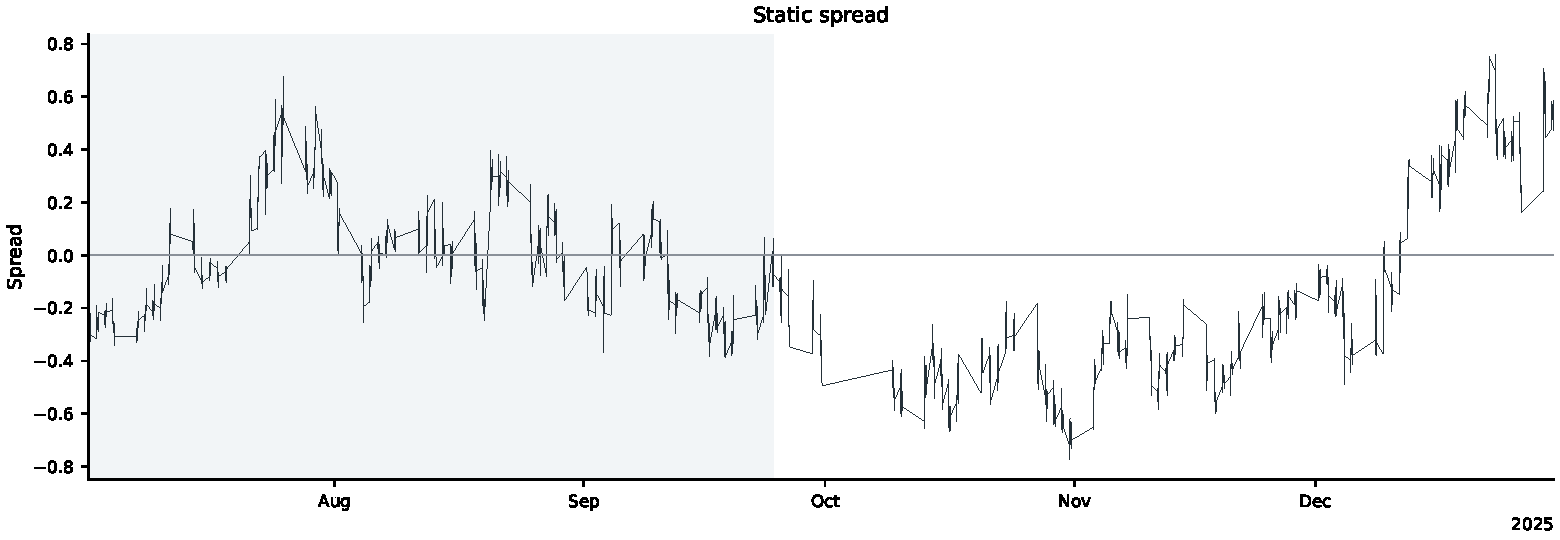
\includegraphics[width=\textwidth]{figures/stage1_static_spread.pdf}
\caption{Static spread, one-minute lasts, 1 July through 30 December 2025. The shaded band is the training window.}
\label{fig:static-spread}
\end{figure}

The rolling OLS fit refits $\alpha$ and $\beta$ every session on the previous 20 sessions of 1-minute lasts. Over the first three months that beta runs from 0.795 to 1.143.

On the training window the rolling residual reverts faster than the static residual, with a half-life of 200 minutes against 304. The static figure is one OLS fit of the AR(1) on that residual, 14{,}756 pairs: $a = 0.99772$, $\mu = -0.027$, $\sigma = 0.0147$, and $\sigma_{\mathrm{eq}} = 0.218$.

Both hedges were then traded with the same trailing-OLS OU estimator of Section~\ref{sec:trailing}. The rolling symmetrical book returns 0.315\% with a Sharpe ratio of 4.31; the static symmetrical book returns 0.827\% with a Sharpe ratio of 8.57. So it appears that the rolling hedge overadapts to the recent window, eating away the trading edge. The baseline in Table~\ref{tab:hedge} is the static fit, and the hedge stays there for the rest of the note.

\begin{table}[ht]
\centering
\caption{Out-of-sample books on static/rolling hedges with the trailing five-session-OLS OU estimator.}
\label{tab:hedge}
\begin{tabular}{llrrrrr}
\toprule
Hedge & Sides & Return & Ann. & Sharpe & Max DD & Trades \\
\midrule
Static & short & 0.505\% & 2.036\% & 5.81 & $-0.065\%$ & 23 \\
Static & long & 0.321\% & 1.292\% & 5.93 & $-0.056\%$ & 17 \\
Static & symmetrical & 0.827\% & 3.347\% & 8.57 & $-0.067\%$ & 40 \\
Rolling & short & 0.155\% & 0.622\% & 2.87 & $-0.105\%$ & 12 \\
Rolling & long & 0.208\% & 0.836\% & 3.72 & $-0.132\%$ & 13 \\
Rolling & symmetrical & 0.315\% & 1.267\% & 4.31 & $-0.156\%$ & 24 \\
\bottomrule
\end{tabular}
\end{table}

\FloatBarrier
\section{Trailing OLS}
\label{sec:trailing}

Through the test, $\mu$, $\sigma$, and $\theta$ are re-estimated every 180 completed one-minute bars. The window is the trailing five sessions, 1{,}200 one-minute bars, and the regression is the session-safe AR(1) of Section~\ref{sec:ou} (no overnight or over-lunch $\Delta t$). The new parameters apply from one minute after the last bar in the window. A window whose AR(1) coefficient falls outside $(0,1)$ keeps the previous fit. All 85 windows on the static spread stay inside $(0,1)$. The entry band is fixed at 2 and the exit band at 0.5.

\section{Kalman filter}

The filter estimates the AR(1) coefficients of the static spread. The hedge stays at the static fit. The state is the pair $(a_t, b_t)$, modelled as a random walk, and the measurement is the next one-minute print of the spread,
\begin{equation}
\begin{pmatrix} a_t \\ b_t \end{pmatrix}
=
\begin{pmatrix} a_{t-1} \\ b_{t-1} \end{pmatrix}
+ w_t,
\qquad
S_t = a_t S_{t-1} + b_t + v_t.
\end{equation}
The process noise $w_t$ has diagonal covariance $\mathrm{diag}(q_a, q_b)$. The measurement noise $v_t$ has variance $R$.

$R$ is the variance of that measurement noise. It is the residual variance of the training-window AR(1), and it stays at that number for the whole run, through the test as well as the training window. On the 14{,}756 training pairs the residual standard deviation is $\sigma_\varepsilon = 0.01469$, so
\[
R = \sigma_\varepsilon^2 = 2.158\times 10^{-4}.
\]
$P_0$ is the covariance of the state at the first minute. It is the OLS sampling covariance of the same two coefficients, $\sigma_\varepsilon^2 (X^{\top} X)^{-1}$, where the columns of $X$ are the lagged spread and a constant:
\[
P_0 =
\begin{pmatrix}
3.678\times 10^{-7} & -2.100\times 10^{-11} \\
-2.100\times 10^{-11} & 1.463\times 10^{-8}
\end{pmatrix}.
\]
The state starts at that fit, $a = 0.99772$ and $b = -6.132\times 10^{-5}$. After each update, $\hat a$ is clipped to $[0.001, 0.999]$. The value stored on a minute is the state from before that minute's print. A lunch gap or an overnight gap carries the previous posterior forward and does not add process noise. $R$ and $P_0$ stay at the training fit, and the filter is carried forward through the test.

The search may change the process noise and the band rule. $R$, $P_0$, the initial state, and the hedge stay at the training fit. The bands move with the filter,
\begin{equation}
z_t = z_0
\left(\frac{\tau_{1/2,t}}{\bar\tau_{1/2}}\right)^{\gamma_\tau}
\left(\frac{\sigma_t}{\bar\sigma}\right)^{\gamma_\sigma},
\end{equation}
with a separate $(z_0, \gamma_\tau, \gamma_\sigma)$ for entry and for exit. $\tau_{1/2} = \ln 2 / \theta$, and $\sigma$ is the diffusion coefficient, both taken from that trial's filter path. The anchors $\bar\tau_{1/2}$ and $\bar\sigma$ are the medians of the in-sample minute path, and the out-of-sample book keeps those training medians. At the anchors the factors equal one, so the band equals $z_0$. An elasticity of zero leaves its factor at one for the whole path. A positive elasticity raises the band when the half-life or $\sigma$ is above its anchor and lowers the band when it is below.

Each of the eight quantities is drawn from the closed interval in Table~\ref{tab:search}. The two logarithmic bounds limit how fast $a$ and $b$ may wander. The elasticities stop at 0.6, so a doubling of the half-life or of $\sigma$ can multiply a band by at most $2^{0.6} \approx 1.52$.

\begin{table}[ht]
\centering
\caption{Box constraints. Each searched quantity is drawn from this interval.}
\label{tab:search}
\begin{tabular}{llc}
\toprule
Parameter & Role & Range \\
\midrule
$\log_{10} q_a$ & process variance of $a$ & $[-10,\,-5]$ \\
$\log_{10} q_b$ & process variance of $b$ & $[-8,\,-3]$ \\
$z_0$ entry & entry band at the anchors & $[1.2,\,2.5]$ \\
$z_0$ exit & exit band at the anchors & $[0.1,\,0.6]$ \\
$\gamma_\tau$ entry & entry elasticity to the half-life & $[0,\,0.6]$ \\
$\gamma_\tau$ exit & exit elasticity to the half-life & $[0,\,0.6]$ \\
$\gamma_\sigma$ entry & entry elasticity to $\sigma$ & $[0,\,0.6]$ \\
$\gamma_\sigma$ exit & exit elasticity to $\sigma$ & $[0,\,0.6]$ \\
\bottomrule
\end{tabular}
\end{table}

Three further bounds are applied to the bands after the formula, on every minute (Table~\ref{tab:bounds}). The entry band is raised to 1 when the formula prints a smaller number. The exit band is raised to 0.05 when the formula prints a smaller number. The exit band is then capped at 0.8 below the entry band. These bounds are the same for every trial. At the anchors, a trial with $z_0$ entry $= 1.2$ and $z_0$ exit $= 0.6$ therefore trades an exit of 0.4.

\begin{table}[ht]
\centering
\caption{Bounds applied to both bands after the formula, on every minute.}
\label{tab:bounds}
\begin{tabular}{ll}
\toprule
Bound & Rule \\
\midrule
Entry floor & $z^{\mathrm{entry}} \ge 1$ \\
Exit floor & $z^{\mathrm{exit}} \ge 0.05$ \\
Gap & $z^{\mathrm{entry}} - z^{\mathrm{exit}} \ge 0.8$ \\
\bottomrule
\end{tabular}
\end{table}

The training sessions are split into three chronological blocks of 21, 21, and 20 sessions: 1--29 July, 30 July--27 August, and 28 August--24 September. Each block's symmetrical book starts flat. Let $S_1$, $S_2$, and $S_3$ be the Sharpe ratios of those three books. The search maximises
\begin{equation}
J = \bar S - s,
\qquad
\bar S = \frac{S_1 + S_2 + S_3}{3},
\qquad
s = \sqrt{\frac{(S_1 - \bar S)^2 + (S_2 - \bar S)^2 + (S_3 - \bar S)^2}{3}}.
\end{equation}
$J$ is high when the three blocks each have a high Sharpe and those three numbers lie close together. An Optuna TPE search of 300 trials, the first 40 drawn at random, chooses the trial in Table~\ref{tab:chosen}.

\begin{table}[ht]
\centering
\caption{Trial chosen on the training window, and the objective it scored.}
\label{tab:chosen}
\begin{tabular}{lr}
\toprule
Quantity & Value \\
\midrule
$\log_{10} q_a$ & $-5.10$ \\
$q_a$ & $7.95\times 10^{-6}$ \\
$\log_{10} q_b$ & $-5.65$ \\
$q_b$ & $2.23\times 10^{-6}$ \\
$z_0$ entry & 2.421 \\
$z_0$ exit & 0.508 \\
$\gamma_\tau$ entry & 0.507 \\
$\gamma_\tau$ exit & 0.085 \\
$\gamma_\sigma$ entry & 0.425 \\
$\gamma_\sigma$ exit & 0.187 \\
\midrule
Sharpe, 1--29 July & 13.13 \\
Sharpe, 30 July--27 August & 13.08 \\
Sharpe, 28 August--24 September & 15.85 \\
Mean Sharpe $\bar S$ & 14.02 \\
Std.\ dev.\ $s$ & 1.29 \\
Objective $J$ & 12.73 \\
\bottomrule
\end{tabular}
\end{table}

The chosen $\log_{10} q_a = -5.10$ lies near the top of $[-10, -5]$, so $a$ is given nearly the largest process variance the box allows. $\log_{10} q_b = -5.65$ lies inside $[-8, -3]$. The anchor entry 2.421 is close to the top of $[1.2, 2.5]$, and the anchor exit 0.508 is inside $[0.1, 0.6]$. The gap between those two anchor levels is 1.91, already wider than the required 0.8, so the gap bound does not move them. The entry elasticities, 0.507 on the half-life and 0.425 on $\sigma$, make the entry band widen when reversion is slow and when the diffusion coefficient is large. The exit elasticities, 0.085 and 0.187, leave the exit band nearly still.

\section{Out of sample}

The Kalman symmetrical book is ahead of the trailing book, 1.868\% and a Sharpe ratio of 10.50 against 0.827\% and 8.57, on 227 round trips against 40.

\begin{table}[ht]
\centering
\caption{Out-of-sample books on the static hedge, 25 September through 30 December 2025.}
\label{tab:oos}
\begin{tabular}{llrrrrr}
\toprule
Estimator & Sides & Return & Ann. & Sharpe & Max DD & Trades \\
\midrule
Trailing OLS & short & 0.505\% & 2.036\% & 5.81 & $-0.065\%$ & 23 \\
Trailing OLS & long & 0.321\% & 1.292\% & 5.93 & $-0.056\%$ & 17 \\
Trailing OLS & symmetrical & 0.827\% & 3.347\% & 8.57 & $-0.067\%$ & 40 \\
Kalman & short & 0.983\% & 3.991\% & 7.38 & $-0.120\%$ & 126 \\
Kalman & long & 1.076\% & 4.376\% & 10.49 & $-0.047\%$ & 105 \\
Kalman & symmetrical & 1.868\% & 7.684\% & 10.50 & $-0.123\%$ & 227 \\
\bottomrule
\end{tabular}
\end{table}

Figure~\ref{fig:spread} plots the static spread and the two $z$-scores. Figure~\ref{fig:position} plots the symmetrical positions. Both figures are one-minute lasts. The spread drifts up through December. The trailing $z$-score follows that drift on the 180-minute clock; the Kalman $z$-score, and its entry band, move every minute. The position plot is the consequence: the trailing book holds for hours or days, and the Kalman book is in and out within the session. Positive lots are a short spread.

\begin{figure}[ht]
\centering
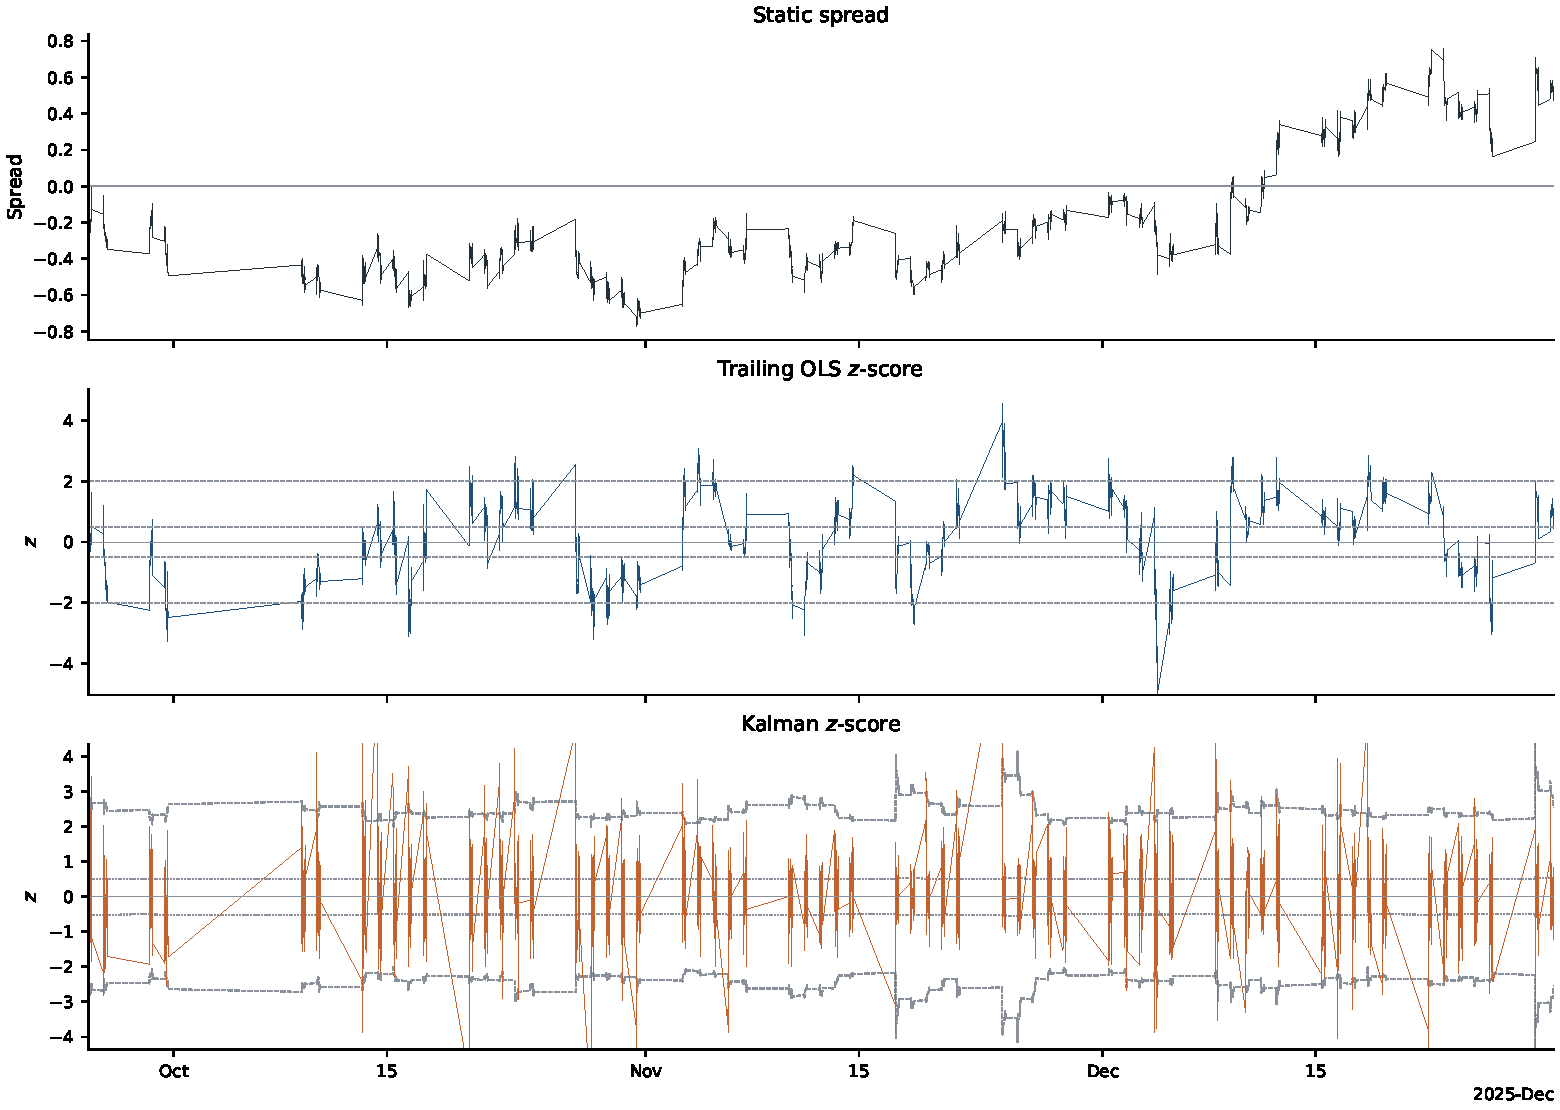
\includegraphics[width=\textwidth]{figures/stage1_oos_spread_z.pdf}
\caption{Out-of-sample static spread and $z$-scores. In the trailing panel the dashed lines are the fixed bands at $\pm 2$ and $\pm 0.5$. In the Kalman panel the dashed lines are the dynamic entry band and the dotted lines are the exit band. The frame follows the body of each series. The trailing $z$-score reaches $-7.2$ on 4 December and the Kalman $z$-score reaches $12.4$; both are clipped.}
\label{fig:spread}
\end{figure}

\begin{figure}[ht]
\centering
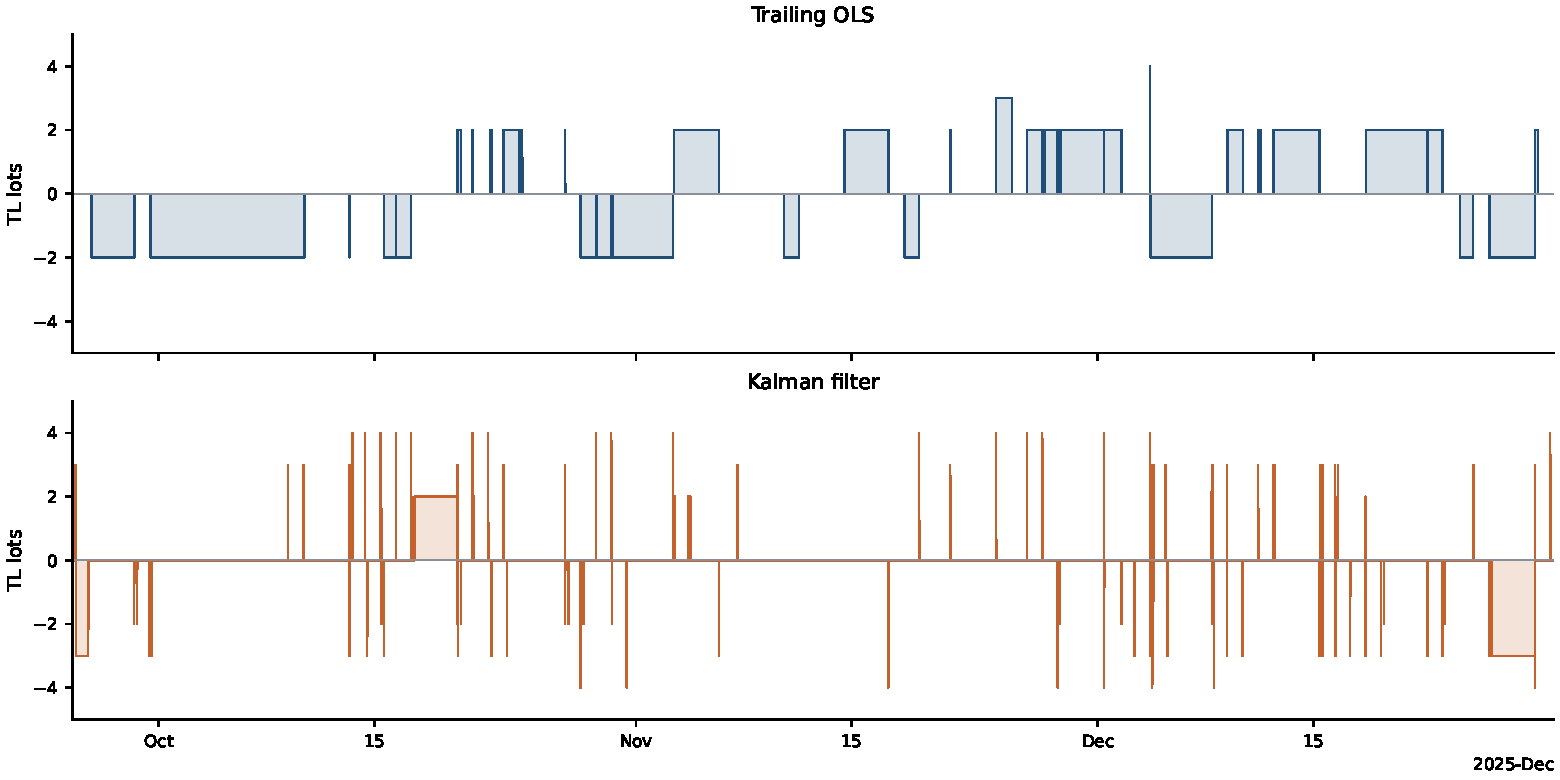
\includegraphics[width=\textwidth]{figures/stage1_oos_positions.pdf}
\caption{Signed TL lots of the symmetrical books. Positive lots are short the spread. The size cap is 8 lots; the trailing book reaches 4 and the Kalman book reaches 4.}
\label{fig:position}
\end{figure}

\end{document}
